\begin{figure}[htbp]
    \caption{Impact of Departures on Others by Intensive Margin Communication History and Involvement}
    \label{fig:prs_opened_comm_int_marg}
    \centering
    \begin{minipage}[b]{0.49\textwidth}
        \centering
        \subcaption{Less involved, highly collaborative} \label{fig:predep_prs_opened_high_collab_comm_int_marg_inv0}
        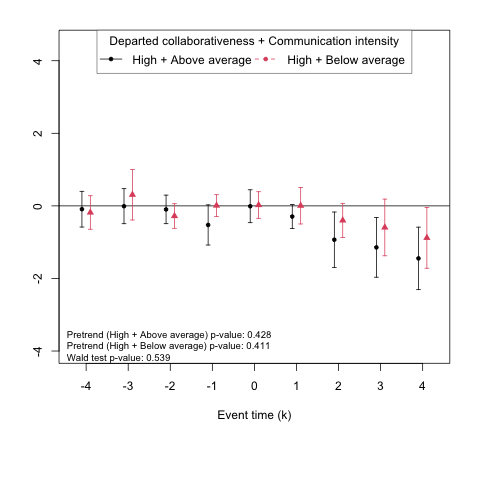
\includegraphics[width=\textwidth]{temp/output/collab_imp/inv0_cs_norm_prs_opened_dept_comm_avg_above_High.png}
    \end{minipage}
    \hfill
    \begin{minipage}[b]{0.49\textwidth}
        \centering
        \subcaption{Less involved, highly collaborative} \label{fig:predep_prs_opened_collab_comm_int_marg_inv0_avg2}
        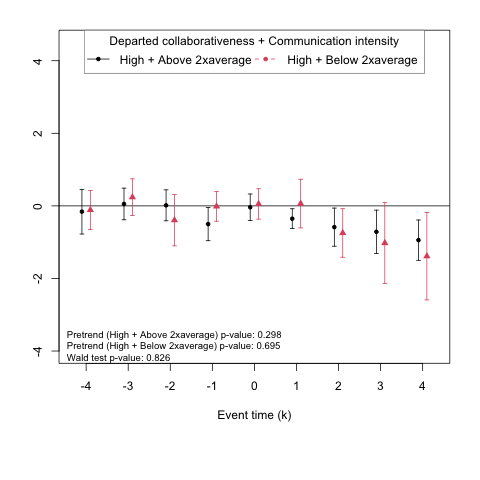
\includegraphics[width=\textwidth]{temp/output/collab_imp/inv0_cs_norm_prs_opened_dept_comm_2avg_above_High.png}
    \end{minipage}
    \begin{minipage}[b]{0.49\textwidth}
        \centering
        \subcaption{Highly involved and collaborative} \label{fig:predep_prs_opened_high_collab_comm_int_marg_inv1}
        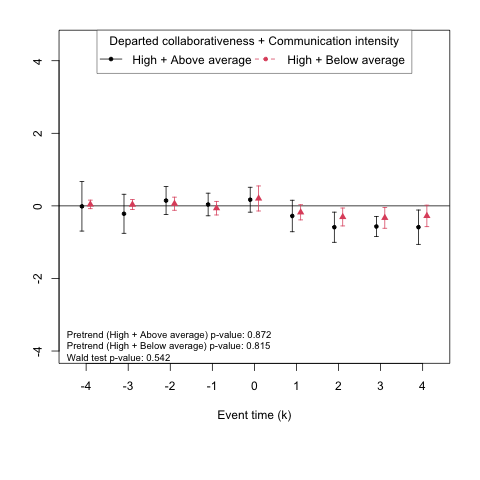
\includegraphics[width=\textwidth]{temp/output/collab_imp/inv1_cs_norm_prs_opened_dept_comm_avg_above_High.png}
    \end{minipage}
    \hfill
    \begin{minipage}[b]{0.49\textwidth}
        \centering
        \subcaption{Highly involved and collaborative} \label{fig:predep_prs_opened_collab_comm_int_marg_inv0_avg1}
        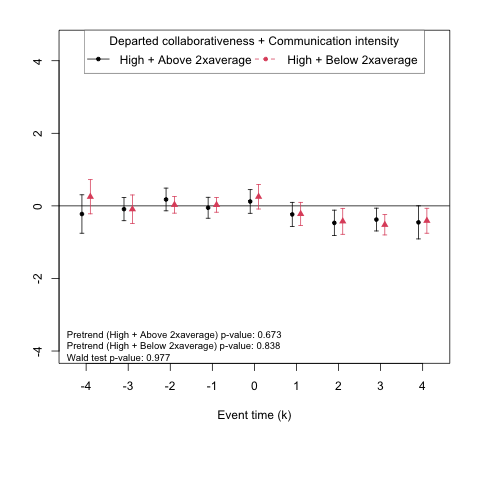
\includegraphics[width=\textwidth]{temp/output/collab_imp/inv1_cs_norm_prs_opened_dept_comm_2avg_above_High.png}
    \end{minipage}
  \begin{minipage}{1\textwidth}
    \textbf{Figure notes:} 
    Following Callaway and Sant’Anna (2021), I estimate event-study coefficients accompanied by 95\% simultaneous confidence bands. For each plot with event study estimates from two subsamples, I report three Wald-test p-values: one for the pretrend test in the first subsample, one for the pretrend test in the second subsample (both from Equation \ref{eq:wald_test_pretrends} in Section \ref{sec:main_method}), and one for the difference in treatment effects across subsamples (Equation \ref{eq:wald_test} in Section \ref{sec:att_subset}). Panel~\subref{fig:predep_prs_opened_high_collab_comm_int_marg_inv0} subsets members based off whether they had \textbf{above average communication intensity with the departed} or \textbf{below average communication intensity with the departed}, as defined in Section~\ref{sec:contr_subset}, conditioning on organizations with highly collaborative and less involved departed members. Panel~\subref{fig:predep_prs_opened_collab_comm_int_marg_inv0_avg2} subsets members based off twice the average communication intensity in a organization. Panel~\subref{fig:predep_prs_opened_high_collab_comm_int_marg_inv1} and Panel~\subref{fig:predep_prs_opened_collab_comm_int_marg_inv0_avg1} are analogs of Panel~\subref{fig:predep_prs_opened_high_collab_comm_int_marg_inv0} and Panel~\subref{fig:predep_prs_opened_collab_comm_int_marg_inv0_avg2} for organizations with highly collaborative and involved departed members.
  \end{minipage}
  


\end{figure}
